\subsection{Perceptron classifier}

A \textsc{Matlab} class \texttt{perceptronKlassifier} was developed in \textsc{Matlab} following the algorithm presented in the previous section. We can perform the training and prediction phase using the following snippet.
\begin{lstlisting}
% create classifier object
percep = perceptronKlassifier();

% adjust hyper-parameters
percep.lr = 0.5;            % learning rate
percep.max_epochs = 200;    % 1000 by default

% train classifier
percep.learn(train.X, train.t);

% access learning results locally stored in... 
percep.w                % weight vector
percep.total_epochs     % epochs needed for training

% get predicted output and compute its accuracy
y_pred = percep.predict(test.X);
acc = mean( test.t == y_pred );	% accuracy
\end{lstlisting}

\subsubsection{2D visualization}
\begin{figure}[]
	\centering
	\begin{subfigure}[]{0.25\textwidth}
		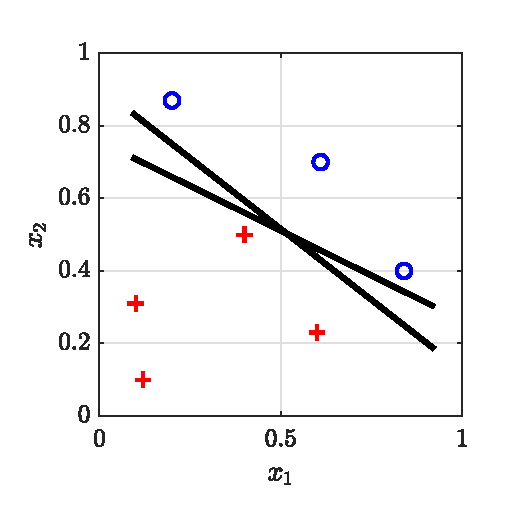
\includegraphics[width=\textwidth]{percep_1a}
		\caption{dataset 1}
		% \label{fig:gull}
	\end{subfigure}%
	%add desired spacing between images, e. g. ~, \quad, \qquad, \hfill etc. 
	%(or a blank line to force the subfigure onto a new line)
	\begin{subfigure}[]{0.25\textwidth}
		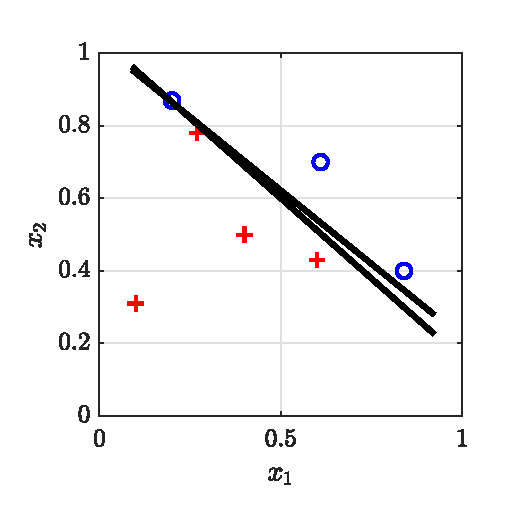
\includegraphics[width=\textwidth]{percep_2a}
		\caption{dataset 2}
		% \label{fig:tiger}
	\end{subfigure}
	\caption{Different linear boundaries found using the perceptron.}
	\label{fig:percep_tests}
\end{figure}

In order to verify that our perceptron works as expected, we train it using two simple 2D datasets and plot the resulting hyperplane. Although results shown in figure \ref{fig:percep_tests} indicate that the perceptron does converge on \textit{some} solution, it has no way of choosing which one is the \textit{best}, which will impact  classification performance when using unseen data. The perceptron of optimal stability, nowadays known as the linear support vector machine was designed to address this problem but it is out of the scope of this report.\\

\subsubsection{Is the semeion-digits dataset linearly separable?}
\begin{figure}[]
	\centering
	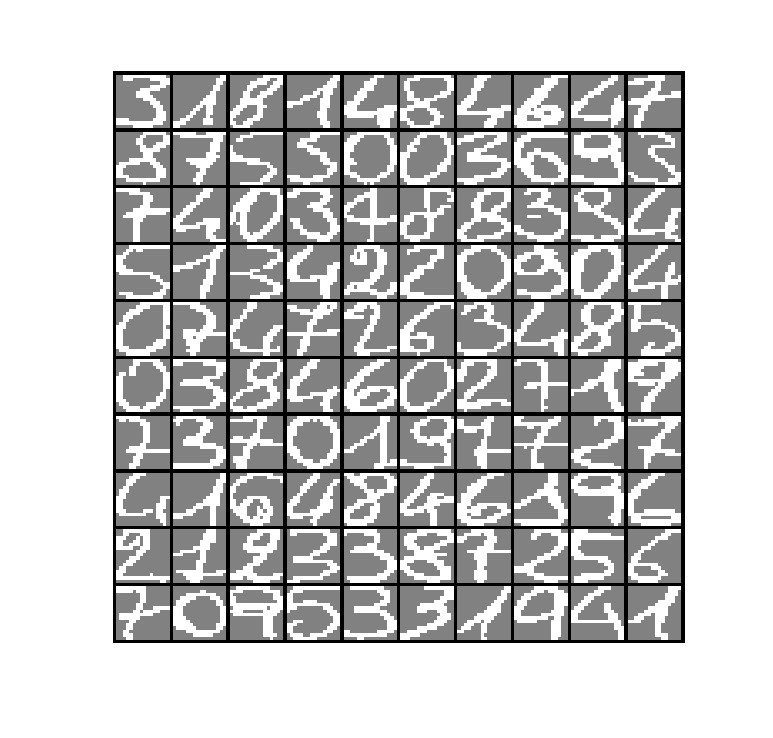
\includegraphics[width=0.4\textwidth, trim={25 25 25 25}, clip]{semeion-digits}
	\caption{Randomly picked samples of the semeion-digits dataset.}
	\label{fig:semeion-digits}
\end{figure}

Since perceptrons work optimally only with linearly separable data, we should ask ourselves: Is the semeion-digits data linearly separable? Then answer is \textit{yes} and the solution was found by training 10 perceptrons using the one-vs-all approach. Each one of them succeeded in finding a linear boundary to separate the given binary classes in a finite number of epochs (table \ref{tbl:epochs_per_class}).
\begin{table}[]
	% increase table row spacing, adjust to taste
	\renewcommand{\arraystretch}{1.3}
	\caption{Epochs needed to linearly separate each class (one-vs-all)}
	\label{tbl:epochs_per_class}
	\centering
	\begin{tabular}{|c||c|c|c|c|c|c|c|c|c|c|}
		\hline
		Digit & 0 & 1 & 2 & 3 & 4 & 5 & 6 & 7 & 8 & 9 \\ \hline 
		Epochs & 10 & 43 & 22 & 32 & 24 & 21 & 21 & 38 & \color{red}187\color{black} & 38 \\ \hline 
	\end{tabular}
\end{table}

\subsection{Cross-validation}
The \textsc{Matlab} function \texttt{cross\_val\_score} was created in order to simplify code structure. It takes as inputs a classifier object, the training set and the number of folds. Outputs the scores in a \textit{struct} containing the performance metrics for each fold, the $k$ trained classifiers and the $k$ chunks of the split data. A simple snippet is provided to show its easy use.
\begin{lstlisting}
knn = kNNKlassifier(5);    % k=5
percep = perceptronKlassifier();

[train, ~] = stratified_split(X, t, 1);

kFolds = 5;
[knn_scores, ~] = cross_val_score(knn, ...
    train.X, train.t, kFolds);
[percep_scores, ~] = cross_val_score(percep, ...
    train.X, train.t, kFolds);
\end{lstlisting}

\subsubsection{How does the number of folds influence the classifier performance?}
%\begin{figure}[]
%	\centering
%	\begin{subfigure}[]{0.25\textwidth}
%		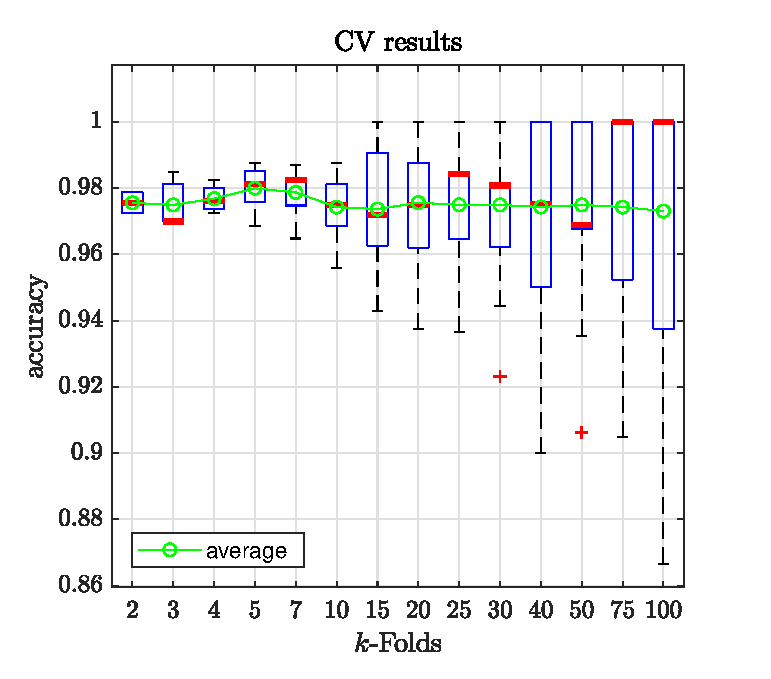
\includegraphics[width=\textwidth]{knn_CV_scores_1}
%		\caption{$k$-NN classifier}
%		 \label{fig:gull}
%	\end{subfigure}%
%	add desired spacing between images, e. g. ~, \quad, \qquad, \hfill etc. 
%	(or a blank line to force the subfigure onto a new line)
%	\begin{subfigure}[]{0.25\textwidth}
%		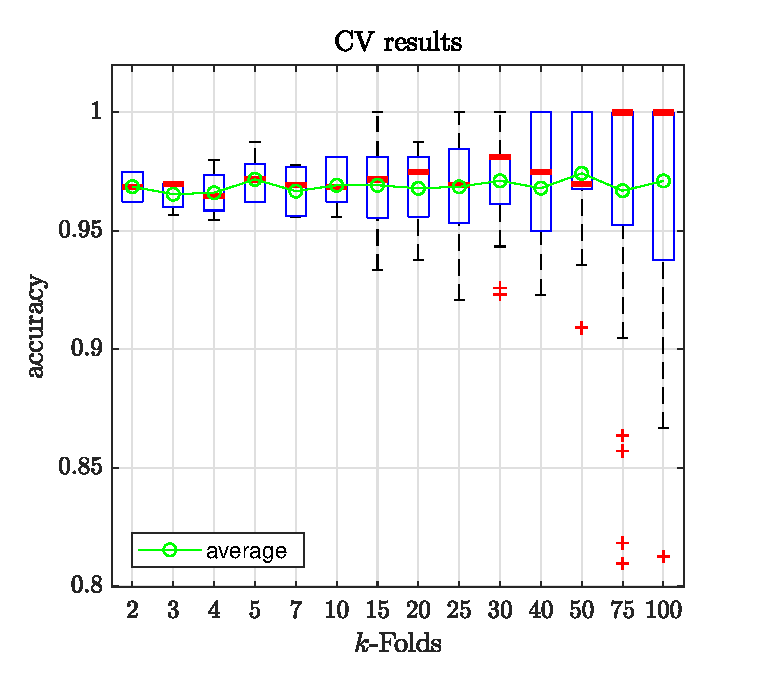
\includegraphics[width=\textwidth]{prc_CV_scores_1}
%		\caption{Perceptron classifier}
%		\label{fig:tiger}
%	\end{subfigure}
%	\caption{Accuracy box plots of CV results (varying number of folds).}
%	\label{fig:CV_scores_1}
%\end{figure}
\begin{figure}
	\centering
	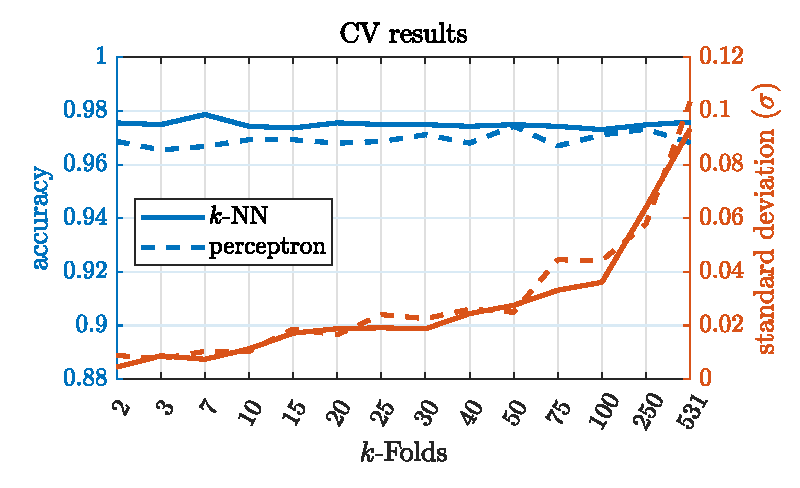
\includegraphics[width=0.45\textwidth]{CV_scores_0}
	\caption{Cross-validation results varying number of folds. Note that the left axis corresponds to the accuracy and the right axis to the standard deviation}
	\label{fig:CV_scores_0}
\end{figure}
To get a better understanding on how the number of folds impacts on the classifier performance, we performed the following test:
\begin{enumerate}
	\item Use the whole dataset as training set
	\item Binarize target vector using digit \textit{1} as target class.
	\item Fix hyper-parameters, if any, of the classifiers to be tested.
	\item Perform CV with the $k$-NN and perceptron classifiers increasing the number of folds progressively.
	\item Plot performance results in the form of box plots, which is a compact way of graphically representing data distribution.
\end{enumerate}

Cross-validation wasn't designed for improving accuracy itself but rather to obtain a general model to use on unseen data. For choosing a good value of $k$ we must minimize \textit{variance} and \textit{bias}. When having a large number of folds we're left out with less observations for testing, thus predictions are more sensitive to misclassification and, in turn, we get higher variance as shown in figure \ref{fig:CV_scores_0}. A small number of folds isn't the solution either since we don't want to hold-out too much of the data (high bias) for testing. It seems that keeping the number of folds around $10$ is a good variance-bias trade-off while ensuring that the classifier itself has low bias and variance.\\

\subsubsection{Leave-one-out cross-validation}
\begin{table}[]
	% increase table row spacing, adjust to taste
	\renewcommand{\arraystretch}{1.3}
	% if using array.sty, it might be a good idea to tweak the value of
	% \extrarowheight as needed to properly center the text within the cells
	\caption{LOOCV results using whole dataset}
	\label{tbl:LOOCV_res}
	\centering
	% Some packages, such as MDW tools, offer better commands for making tables
	% than the plain LaTeX2e tabular which is used here.
	% 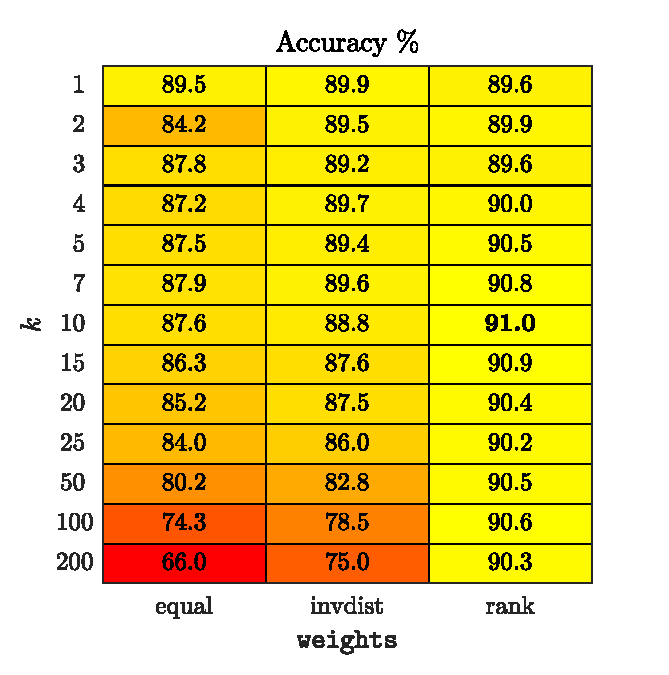
\includegraphics[width=0.4\textwidth]{knn_gridsearchCV_1}
	\begin{tabular}{|c||c|c|}
		\hline
		& accuracy & standard deviation \\ \hline \hline
		$k$-NN       &  0.9743  &   0.1584 \\ \hline
		perceptron   &  0.8983  &   0.3023 \\ \hline
	\end{tabular}
\end{table}
LOOCV can be seen as a special case of $k$-fold CV when $k$ equals the total number of observations in the training set. This approach requires excessive computation and provides the most variance since, at each fold, accuracy can only be either 100\% or 0\%. Nonetheless, this turns out to be handy for analyzing the percentage of outliers or hard samples in the dataset. From table \ref{tbl:LOOCV_res}, the outlier percentage can be obtained from the complement of accuracy (error percentage) where $k$-NN outperforms the perceptron. 
% TODO: analyze leave-one-out cross-validation (LOOCV)

\subsubsection{Adjusting hyper-parameters with CV}
Cross-validation was initially designed as a method to train a classifier such that we end up with a \text{generalized} model before it's let out into the world. This generalization is achieved by fine-tuning the classifier's hyper-parameters.

Since the standard perceptron algorithm aforementioned has no hyper-parameters there is not much we can do to enhance its performance when testing it with unseen data. On the other hand, the implemented $k$-NN algorithm has the following hyper-parameters:
\begin{itemize}
	\item \texttt{k}: number of $k$-nearest neighbors used to classify unseen data. Can take any value from 1 to the total number of observations in training set.
	\item \texttt{weighfcn}: defines the weight contribution of each neighbor.
	\begin{itemize}
		\item \texttt{equal}: No weighting
		\item \texttt{invdist}: weight is 1/distance
		\item \texttt{rank}: weight is 1/rank
	\end{itemize}
\end{itemize}

Using 50\% of the dataset for CV tuning and 50\% for blind validation, we performed an exhaustive search (also referred to as CV grid search) over specified hyper-parameter values for the $k$-NN classifier. Average accuracy results, using 5x5CV (5 iterations of 5-fold cross-validation) on each hyper-parameter combination, are displayed in figure \ref{tbl:knn_gridsearchCV}. Accuracy tends to decrease when taking into account a large number of neighbors except when using \texttt{rank} for weighting contributions. The hyper-parameters [$k$, \texttt{weighfcn}] that yield the highest average accuracy of $90.951$\% is [10, \texttt{rank}]. Alternative performance metrics show the same behavior:
\begin{itemize}
	\item Highest average precision score: $0.916 \gets$ [$10$, \texttt{rank}]
	\item Highest average recall score: $0.909 \gets$ [$10$, \texttt{rank}]
	\item Highest average F1 score: $0.908 \gets$ [$10$, \texttt{rank}]
\end{itemize}
We'll therefore choose these hyper-parameters for further testings and comparisons.
%\begin{table}[]
%	% increase table row spacing, adjust to taste
%	\renewcommand{\arraystretch}{1.3}
%	% if using array.sty, it might be a good idea to tweak the value of
%	% \extrarowheight as needed to properly center the text within the cells
%	\caption{$k$-NN average accuracy results using 5x5CV gridsearch.}
%	\label{tbl:knn_gridsearchCV}
%	\centering
%	% Some packages, such as MDW tools, offer better commands for making tables
%	% than the plain LaTeX2e tabular which is used here.
%	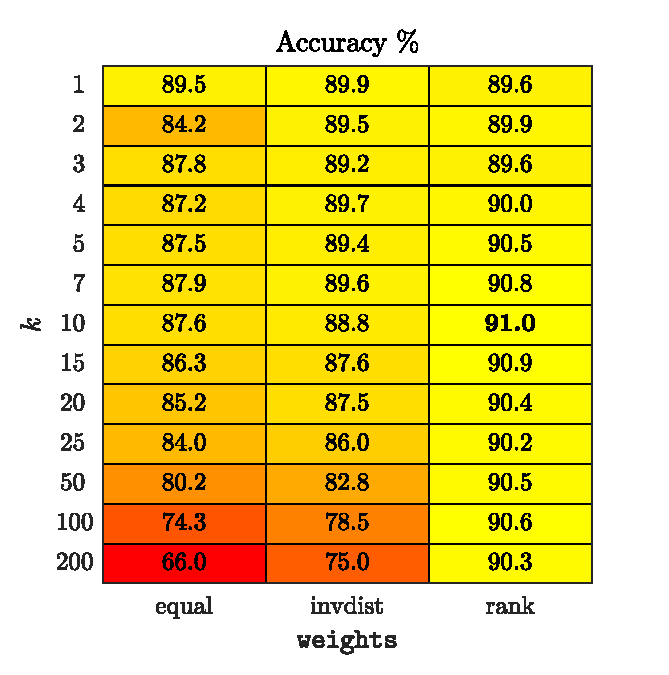
\includegraphics[width=0.4\textwidth]{knn_gridsearchCV_1}
%%	\begin{tabular}{|c||c|c|c|}
%%		\hline
%%		k \textbackslash weighfcn  & \texttt{equal} & \texttt{invdist} & \texttt{rank} \\ \hline \hline
%%		1   &  0.8950 &   0.8969 &   0.8958 \\ \hline
%%		2   &  0.8422 &   0.8895 &   0.8935 \\ \hline
%%		3   &  0.8777 &   0.8915 &   0.8966 \\ \hline
%%		4   &  0.8721 &   0.9001 &   0.9042 \\ \hline
%%		5   &  0.8755 &   0.8962 &   0.9083 \\ \hline
%%		7   &  0.8790 &   0.8913 &   0.9105 \\ \hline
%%		10  &  0.8762 &   0.8929 &   0.9062 \\ \hline
%%		15  &  0.8628 &   0.8801 &   0.9033 \\ \hline
%%		20  &  0.8516 &   0.8705 &   0.9073 \\ \hline
%%		25  &  0.8404 &   0.8573 &   0.9080 \\ \hline
%%		50  &  0.8025 &   0.8286 &   0.9052 \\ \hline
%%		100 &  0.7433 &   0.7864 &   0.9043 \\ \hline
%%		200 &  0.6603 &   0.7434 &   0.9035 \\ \hline
%%	\end{tabular}
%\end{table}
\begin{figure}
	\centering
	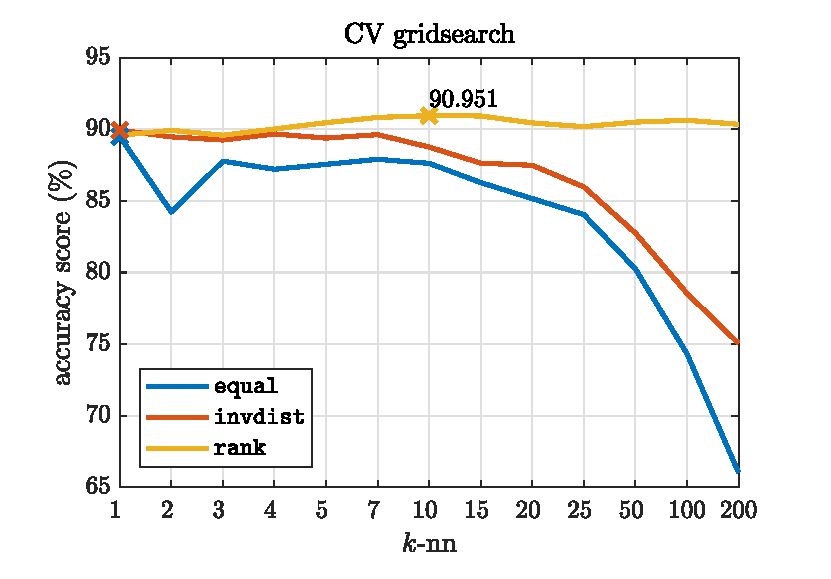
\includegraphics[width=0.45\textwidth]{knn_gridsearchCV_0}
	\caption{$k$-NN average accuracy results using 5x5CV grid search.}
	\label{tbl:knn_gridsearchCV}
\end{figure}

\subsection{Perceptron vs $k$-NN algorithm}
So far we have two classification models and we would like to compare their results. These classifiers are quite different from one another, the main difference being their training and testing phase. The perceptron carries out  most of the heavy computing at the training phase, contrary to the $k$-NN algorithm (lazy-learner) where all the computation is left to the predicting phase. We're particularly interested in knowing how well our classifiers perform on predicting true positives, therefore we'll mainly use \textit{recall}, \textit{precision} and \textit{F1} scores to measure and compare their performance.\\

\subsubsection{Binarized targets}
\begin{table}[]
	% increase table row spacing, adjust to taste
	\renewcommand{\arraystretch}{1.3}
	% if using array.sty, it might be a good idea to tweak the value of
	% \extrarowheight as needed to properly center the text within the cells
	\caption{$k$-NN average performance scores (5x10CV)}
	\label{tbl:knn_perf_scores}
	\centering
	% Some packages, such as MDW tools, offer better commands for making tables
	% than the plain LaTeX2e tabular which is used here.
	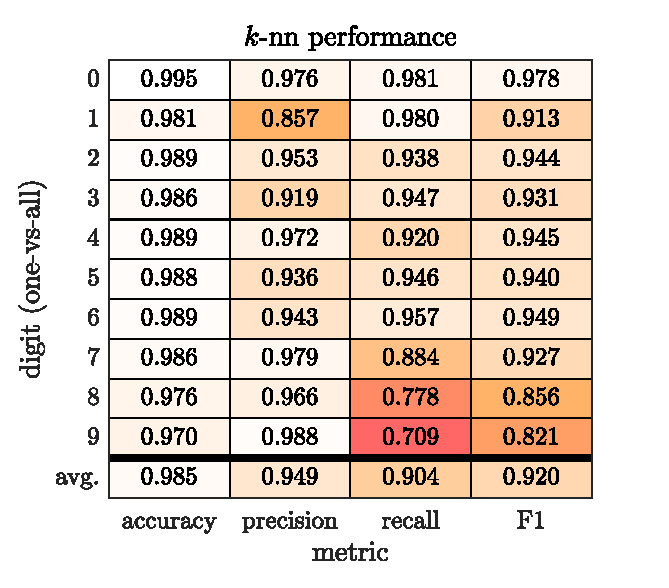
\includegraphics[width=0.4\textwidth]{knn_perf_scores}
\end{table}

\begin{table}[]
	% increase table row spacing, adjust to taste
	\renewcommand{\arraystretch}{1.3}
	% if using array.sty, it might be a good idea to tweak the value of
	% \extrarowheight as needed to properly center the text within the cells
	\caption{Perceptron average performance scores (5x10CV)}
	\label{tbl:percep_perf_scores}
	\centering
	% Some packages, such as MDW tools, offer better commands for making tables
	% than the plain LaTeX2e tabular which is used here.
	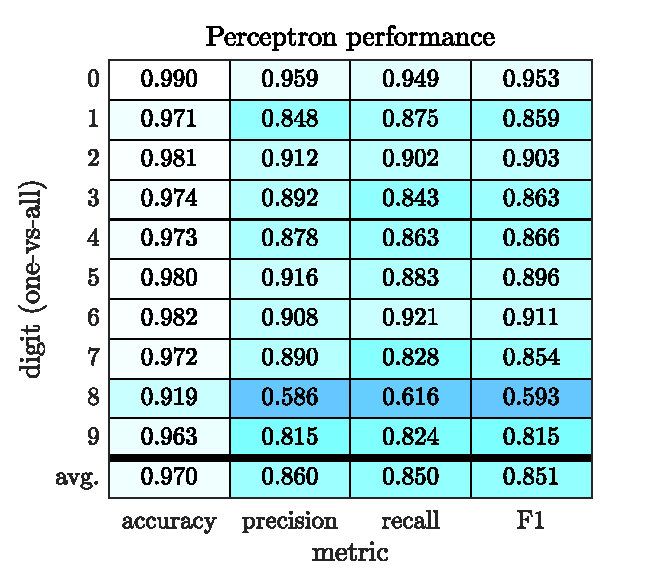
\includegraphics[width=0.4\textwidth]{percep_perf_scores}
\end{table}

Both classifiers are able to predict binary outputs, which is the simplest case of a classification problem. In order to obtain results as neutral as possible, we used all the available data and performed 5x10CV. Results then were averaged and are presented in tables \ref{tbl:knn_perf_scores} and \ref{tbl:percep_perf_scores}. Each row is independent from one another since for each digit we performed a one-vs-all binarization. 

In the $k$-NN case, precision and recall show some mayor differences between one another. Taking digit $9$ as an example, we get a small number of false positives (high precision) but we have a large number of false negatives (low recall); in other words, whenever $k$-NN predicts a $9$ we can be pretty confident the number is an actual $9$, however, when the prediction is \textit{not a $9$} there is 30\% chance the prediction is mistaken. Digit $1$ presents an inverse behavior; we're confident when prediction is \textit{not a $1$}, but other digits may be falsely classified as $1$.

Focusing now on the perceptron performance, precision and recall present a similar score for all binary outputs. Meaning that regardless of the prediction output, we'll always have some uncertainty on it; specially for digit $8$ where the chance of getting a wrong prediction is 40\%.

Both classifiers show high average accuracy, but when referring to other metrics the panorama changes. Unbalanced class proportion is the main reason for this behavior. The F1 column can be seen as a weighted average of precision and recall, giving us a good picture of the overall performance.\\

\subsubsection{Multiclass classification}
Is there a way to know which pair of digits get confused with one another? Previously, we had no way of knowing if the classifier was confusing two of the 10 available classes. With multiclass classification we're able to predict between more than two categories $y = \lbrace 0, 1, ... n \rbrace$. Then, we can use this prediction to plot a \textit{confusion matrix}, which is a powerful tool for visualizing algorithm's performance. The name stems from the fact that it makes it easy to see if the system is confusing two classes.

The $k$-NN algorithm requires no modification since it handles both binray and multiclass classification in the same way. 

The perceptron is by nature a binary classifier, therefore we divide our problem into $n+1$ binary classification problems; in each one, we predict the probability that $y$ is a member of one of $n$ classes and then use the perceptron that returned the highest value as our prediction \cite{coursera-ML}. In our case, the use of \textit{sign} as an activation function doesn't output a probability, instead we'll take the weighted sum to compare and choose the highest.
\begin{gather*}
y \in \left\lbrace 0, 1, ... 9 \right\rbrace  \\
h^{(0)}(x) = \boldsymbol{w}^{(0)} \boldsymbol{x} \\
h^{(1)}(x) = \boldsymbol{w}^{(1)} \boldsymbol{x} \\
\vdots \\
h^{(9)}(x) = \boldsymbol{w}^{(9)} \boldsymbol{x} \\
\text{prediction} = \max_i(h^{(i)}(x))
\end{gather*}

Once more, we performed 5x10CV and computed a confusion matrix at each step. We then averaged all 50 of them and applied F1 scoring over all the elements as shown in figure \ref{fig:avg_CMats}. One of the first things we notice when looking at the results is that the confusion matrix for the perceptron is \textit{dirtier} in the sense that there are lots of weak misclassifications, whereas the $k$-NN has few but strong confusions between classes.
\begin{figure}[]
	\centering
	\begin{subfigure}[]{0.4\textwidth}
		\centering
		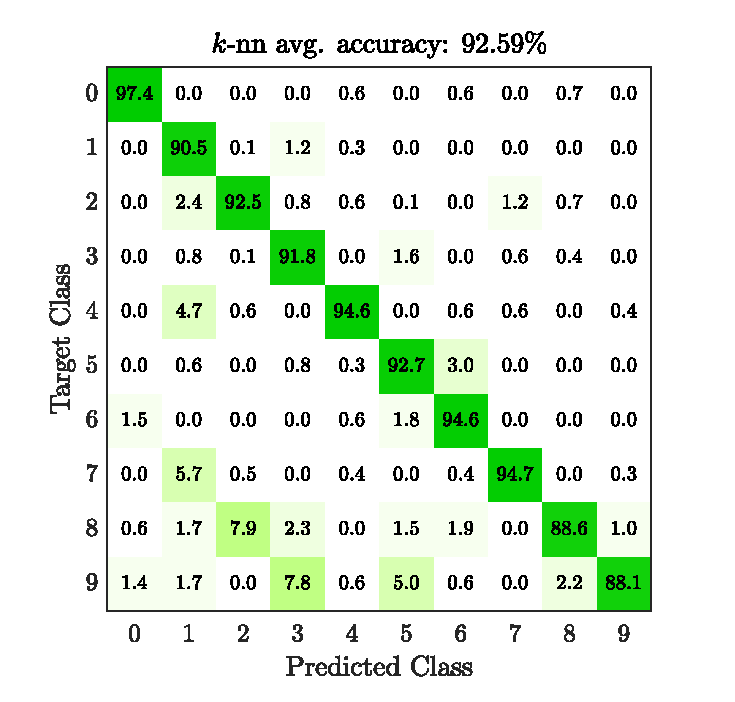
\includegraphics[width=\textwidth]{knn_avgCMat}
		\caption{$k$-NN performance}
		% \label{fig:gull}
	\end{subfigure}
	%add desired spacing between images, e. g. ~, \quad, \qquad, \hfill etc. 
	%(or a blank line to force the subfigure onto a new line)
	\begin{subfigure}[]{0.4\textwidth}
		\centering
		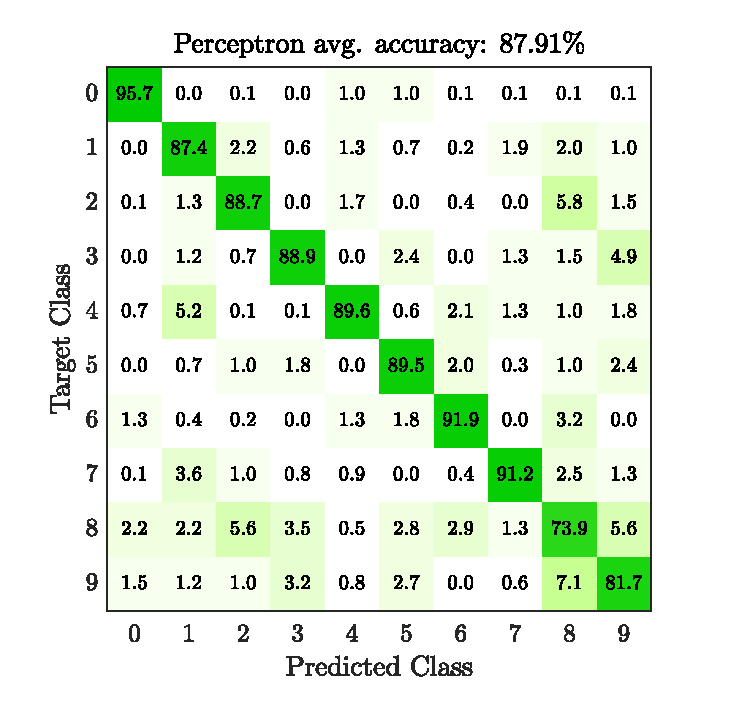
\includegraphics[width=\textwidth]{percep_avgCMat}
		\caption{Perceptron performance}
		% \label{fig:tiger}
	\end{subfigure}
	\caption{Classifiers' confusion matrices with F1 scores.}
	\label{fig:avg_CMats}
\end{figure}

Addressing the overall performance of each classifier, we can point out the following:
\begin{itemize}
	\item $k$-NN classifier
	\begin{itemize}
		\item Strong confusion between $8 \gets 2$ and $9 \gets 3$.
		\item Precision avg. score: 0.933
		\item Recall avg. score: 0.925.
		\item F1 avg. score: 0.926.
	\end{itemize}
	\item Perceptron multiclass classifier
	\begin{itemize}
		\item Strong confusion between $8 \leftrightarrow 2$, $9 \leftrightarrow 8$ $ \gets 1$.
		\item Precision avg. score: 0.884
		\item Recall avg. score: 0.879.
		\item F1 avg. score: 0.878.
		\item Digit $8$ has a poor score and, by looking at table \ref{tbl:epochs_per_class}, we note that the perceptron needs a large number of epochs to find a suitable hyperplane, suggesting that this high dimensional boundary is in a \textit{tight} space (prone to misclassification). On a 2D scenario it would look similar to figure \ref{fig:percep_tests}b.
	\end{itemize}
\end{itemize}
